% Drawing 91/05-1 -- folder 91, batch 05, archive page 83 (PDF page 84).
% Transcription: en haut à gauche, un croquis~: une grande région marquée « \uncertain{qu.~cpt} », contenant deux ouverts qui se recoupent, notés $U_f$ et $U_g$, avec leur intersection notée \uncertain{$U_f \cap U_g$}~; un petit cercle au-dessus, et un cercle barré plus à droite~; un $\overline{X}$ isolé.
% Kind: open sets in a region (Venn sketch). Method 2 (schematic redraw from the facsimile). Status: partial.
% Notes: A large region marked "qu. cpt" (uncertain) containing two overlapping open sets U_f and U_g, their intersection labelled under them; a small circle above, a struck circle further right, and an isolated X-bar. The small labels are placed after the transcription; a small arrow at the left of the region is left out. The faint lines of text across the crop are left out.
% Coordinates: 1 unit = 1 mm = 1/100 of the crop width (bbox in page fractions: [0.08, 0.06, 0.58, 0.26]).
% Redrawn by Claude (claude-opus-5-5), issue #73, 2026-11-07; not checked by a human; not compiled (no TeX in the session).
% Rights: reproduces part of the work -- behind RENDER_TRANSCRIPTS, never published by itself.
\documentclass[tikz,border=3pt]{standalone}
\usepackage{amsmath,amssymb}
\usetikzlibrary{patterns,arrows.meta}
\tikzset{pencil/.style={black!45}, struck/.style={black!35}, mark/.style={circle,draw,inner sep=1.3pt}, pt/.style={circle,fill,inner sep=0.9pt}, opt/.style={circle,draw,fill=white,inner sep=1.1pt}}
\begin{document}
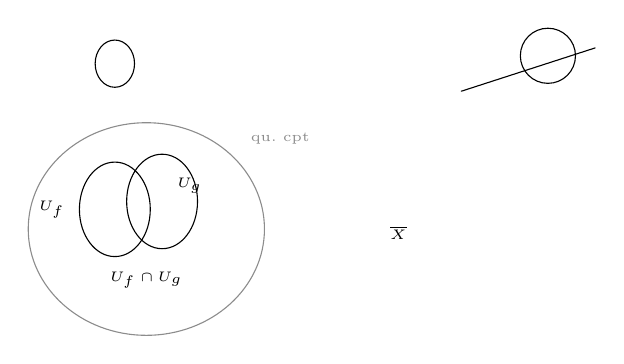
\begin{tikzpicture}[x=1mm,y=1mm,line cap=round,line join=round,font=\scriptsize]
\draw[pencil] (35,-39.5) ellipse[x radius=15, y radius=13.5];
\draw (31,-37) ellipse[x radius=4.5, y radius=6];
\draw (37,-36) ellipse[x radius=4.5, y radius=6];
\node[inner sep=1pt] at (23,-37) {\tiny $U_f$};
\node[inner sep=1pt] at (40.5,-34) {\tiny $U_g$};
\node[inner sep=1pt] at (35,-46) {\tiny $U_f\cap U_g$};
\node[inner sep=1pt,pencil] at (52,-28) {\tiny qu.~cpt};
\draw (31,-18.5) ellipse[x radius=2.5, y radius=3];
\draw (86,-17.5) circle[radius=3.5];
\draw (75,-22) -- (92,-16.5);
\node[inner sep=1pt] at (67,-40) {\tiny $\overline{X}$};
\end{tikzpicture}
\end{document}
